%
% main.tex -- Paper zum Thema <kepler>
%
% (c) 2026 Jan Klarer, Manuel Kuhn, OST Ostschweizer Fachhochschule
%
% !TEX root = ../../buch.tex
% !TEX encoding = UTF-8
%
\chapter{Das dritte keplersche Gesetz\label{chapter:kepler}}
\kopflinks{Das dritte keplersche Gesetz}
\begin{refsection}
\chapterauthor{Jan Klarer und Manuel Kuhn}
\index{Jan Klarer}%
\index{Klarer, Jan}%
\index{Manuel Kuhn}%
\index{Kuhn, Manuel}%

%
% 01_Einleitung.tex -- Historischer Kontext, die drei Gesetze und
% Zielsetzung der Arbeit
%
% !TEX root = ../../buch.tex
% !TEX encoding = UTF-8
%
\section{Die keplerschen Gesetze
\label{kepler:section:einleitung}}
\kopfrechts{Die keplerschen Gesetze}%

Johannes Kepler formulierte zu Beginn des 17.~Jahrhunderts drei Gesetze über die Bewegung der Planeten um die Sonne.
\index{Kepler, Johannes}%
\index{Sonne}%
\index{Planet}%
Er stützte sich dabei auf die Beobachtungsdaten des dänischen Astronomen Tycho Brahe.
Diese Daten waren für die damalige Zeit aussergewöhnlich präzis.
\index{Brahe, Tycho}%
Die ersten beiden Gesetze veröffentlichte Kepler 1609 in der Astronomia Nova \cite{kepler:astronomianova}.
\index{Astronomia Nova}%
Das dritte Gesetz fand er erst zehn Jahre später.
Er publizierte es 1619 in Harmonices Mundi \cite{kepler:harmonices}.
\index{Harmonices Mundi}%
Die drei Gesetze lauten:
\begin{enumerate}
\item
Die Planeten bewegen sich auf elliptischen Bahnen.
In einem gemeinsamen Brennpunkt dieser Ellipsen steht die Sonne.
\index{Ellipse}%
\item
Ein von der Sonne zum Planeten gezogener Fahrstrahl überstreicht in gleichen Zeiten gleich grosse Flächen.
\index{Fahrstrahl}%
\index{Flachensatz@Flächensatz}%
\item
Die Quadrate der Umlaufzeiten zweier Planeten verhalten sich zueinander wie die Kuben der grossen Halbachsen ihrer Bahnellipsen.
\end{enumerate}
Kepler gewann diese Gesetze rein empirisch aus den Beobachtungsdaten.
Eine physikalische Begründung gelang erst Isaac Newton.
\index{Newton, Isaac}%
Er zeigte 1687 in seinen Principia \cite{kepler:principia}, dass alle drei Gesetze aus dem Gravitationsgesetz folgen.
\index{Principa}%
\index{Graviationsgesetz}%

Diese Arbeit leitet das dritte Gesetz mathematisch aus dem Gravitationsgesetz her.
Die ersten beiden Gesetze beschreiben die Bahn eines einzelnen Planeten.
Das dritte Gesetz vergleicht dagegen verschiedene Planeten miteinander.
Es besagt: Der Quotient $T^2/a^3$ hat für alle Körper um dasselbe Zentralgestirn denselben Wert.
Dabei ist $T$ die Umlaufzeit und $a$ die grosse Halbachse der Bahn.
\index{Umlaufzeit}%
In Lehrbüchern wird das Gesetz meist nur für Kreisbahnen hergeleitet.
Für Kreisbahnen genügt nämlich ein einfaches Kräftegleichgewicht.
Reale Planetenbahnen sind aber Ellipsen.
Für Ellipsen führt die Berechnung der Umlaufzeit auf ein reelles Integral.
Dieses Integral lässt sich mit elementaren Mitteln nur mühsam auswerten.
Elementare Zugänge ohne komplexe Analysis finden sich zum Beispiel bei Vogt \cite{kepler:vogt}.

Wir gehen einen anderen Weg und lösen das Integral mit komplexer Integration.
Die nötigen Methoden wurden im ersten Teil dieses Buches entwickelt.
Abschnitt~\ref{kepler:section:grundlagen} stellt zuerst die geometrischen und physikalischen Grundlagen bereit.
Dort leiten wir die Umlaufzeit als Integral über den Polarwinkel her.
Abschnitt~\ref{kepler:section:kreisbahn} behandelt den Spezialfall der Kreisbahn.
Er dient später als Kontrolle für das allgemeine Resultat.
In Abschnitt~\ref{kepler:section:komplex} verwandeln wir das Integral in ein Wegintegral über den komplexen Einheitskreis.
Dieses Wegintegral werten wir mit der Cauchy-Formel für Ableitungen aus.
Zum Schluss prüfen wir das Resultat an realen Bahndaten von Planeten und einem Kometen.

%
% 02_Grundlagen.tex -- Ellipsengeometrie, Drehimpulserhaltung,
% Bahngleichung und die Umlaufzeit als Integral
%
% !TEX root = ../../buch.tex
% !TEX encoding = UTF-8
%
\section{Geometrische und physikalische Grundlagen
\label{kepler:section:grundlagen}}
\kopfrechts{Geometrische und physikalische Grundlagen}%

Für die Umlaufzeit eines Planeten brauchen wir zwei Zutaten.
Die erste Zutat ist die geometrische Form der Bahn.
Die zweite Zutat ist die Geschwindigkeit, mit der der Planet diese Bahn durchläuft.
Die Form liefert das erste keplersche Gesetz.
Die Geschwindigkeit liefert das zweite.
In diesem Abschnitt beschreiben wir zuerst die Ellipse in Polarkoordinaten.
Dann leiten wir beide Gesetze aus der newtonschen Mechanik her.
Daraus gewinnen wir eine Integraldarstellung der Umlaufzeit.
Diese Darstellung ist der Ausgangspunkt für alles Weitere.

\subsection{Die Ellipse in Polarkoordinaten
\label{kepler:subsection:ellipse}}

\begin{figure}
\centering
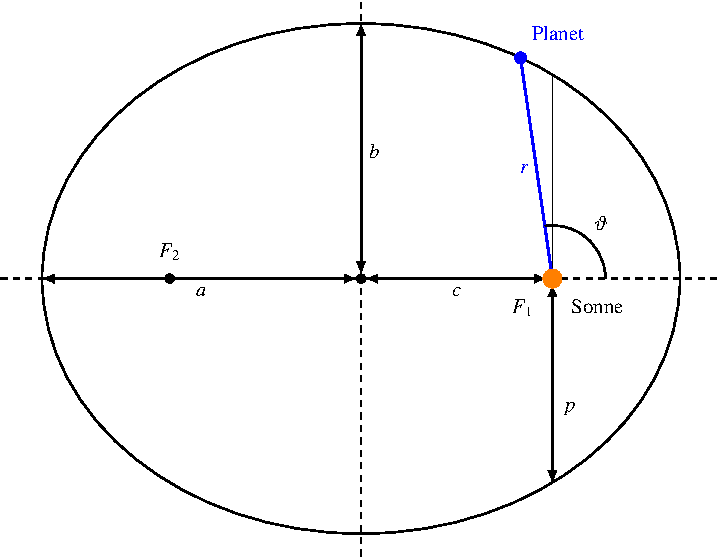
\includegraphics{papers/kepler/images/bahn.pdf}
\caption{Bahnellipse eines Planeten mit grosser Halbachse $a$ und
kleiner Halbachse $b$.
Die Sonne steht im Brennpunkt $F_1$.
Der zweite Brennpunkt $F_2$ bleibt leer.
Die Brennpunkte liegen im Abstand $c$ vom Mittelpunkt der Ellipse.
Der Halbparameter $p$ wird senkrecht zur grossen Achse gemessen.
Die durchgezogene Sehne durch $F_1$ liegt symmetrisch zur grossen Achse und steht deshalb senkrecht auf ihr.
Der Ort des Planeten wird durch den Abstand $r$ zur Sonne und den Polarwinkel $\vartheta$ beschrieben.
Der Winkel wird vom sonnennächsten Punkt aus gemessen.
\label{kepler:figure:ellipse}}
\end{figure}


Eine Ellipse hat eine grosse Halbachse $a$ und eine kleine Halbachse $b$.
\index{Halbachse}%
Sie besitzt zwei Brennpunkte $F_1$ und $F_2$.
\index{Brennpunkt}%
Diese liegen auf der grossen Achse im Abstand $c=\!\sqrt{a^2-b^2}$ vom Mittelpunkt (Abbildung~\ref{kepler:figure:ellipse}).
Das Verhältnis
\begin{equation}
\varepsilon
=
\frac{c}{a}
=
\!\sqrt{1-\frac{b^2}{a^2}}
\label{kepler:eqn:exzentrizitaet}
\end{equation}
heisst \emph{numerische Exzentrizität}.
\index{Exzentriztität, numerisch}%
Sie misst die Abweichung von der Kreisform.
Für eine Ellipse gilt $0\le \varepsilon<1$.
Der Grenzfall $\varepsilon=0$ ergibt einen Kreis.
Wir schreiben die Exzentrizität mit dem griechischen Buchstaben $\varepsilon$.
\index{epsilon@$\varepsilon$}%
Das reguläre $e$ bleibt so für die eulersche Zahl reserviert.
\index{e@$e$}%
\index{eulersche Zahl}%

Für die Rechnung eignen sich Polarkoordinaten $(r,\vartheta)$ am besten.
\index{Polarkoordinaten}%
Die Sonne liegt dabei im Ursprung, also im Brennpunkt $F_1$.
\index{Sonne}%
In diesen Koordinaten lautet die Gleichung der Ellipse
\begin{equation}
r(\vartheta)
=
\frac{p}{1+\varepsilon\cos(\vartheta)}
\qquad\text{mit}\qquad
p
=
\frac{b^2}{a}
=
a(1-\varepsilon^2).
\label{kepler:eqn:ellipse}
\end{equation}
Die Grösse $p$ heisst \emph{Halbparameter} der Ellipse.
\index{Halbparameter}%
\index{p@$p$}%
Sie ist der Abstand von der Sonne zur Bahn senkrecht zur grossen Achse.
Der Winkel $\vartheta$ wird vom sonnennächsten Punkt aus gemessen.
Für $\vartheta=0$ ist der Nenner maximal und der Abstand $r$ minimal.
Für $\vartheta=\pi$ erreicht der Planet den sonnenfernsten Punkt.
In Abschnitt~\ref{kepler:subsection:bahngleichung} leiten wir diese
Bahnform aus der Bewegungsgleichung her.

\subsection{Drehimpulserhaltung und der Flächensatz
\label{kepler:subsection:flaechensatz}}

Die Sonne habe die Masse $M$ und der Planet die Masse $m$.
Nach Newton \cite{kepler:principia} ist die Gravitationskraft
\begin{equation}
\vec{F}
=
-\frac{GMm}{r^2}\,\hat{r}.
\label{kepler:eqn:gravitation}
\end{equation}
Dabei ist $G$ die Gravitationskonstante.
Der Vektor $\hat{r}$ ist der Einheitsvektor von der Sonne zum Planeten.
Die Gravitation ist eine Zentralkraft.
\index{Zentralkraft}%
Sie wirkt immer entlang der Verbindungslinie von Sonne und Planet.
Deshalb verschwindet das Drehmoment bezüglich der Sonne: Wegen
$\vec{F}\parallel\vec{r}$ gilt $\vec{r}\times\vec{F}=0$.
Das Drehmoment ist die zeitliche Änderung des Drehimpulses.
\index{Drehmoment}%
Der Drehimpuls
\index{Drehimpuls}%
\begin{equation}
\vec{L}
=
m\,(\vec{r}\times\vec{v})
=
\text{konstant}
\label{kepler:eqn:drehimpulsvektor}
\end{equation}
bleibt deshalb während der ganzen Bewegung erhalten.
Daraus folgt auch, dass die Bahn eben ist.
Der Ortsvektor $\vec{r}$ steht nämlich immer senkrecht auf dem festen Vektor $\vec{L}$.
Wir können die Bewegung deshalb vollständig in der Bahnebene beschreiben.
\index{Bahnebene}%
Dazu verwenden wir die Polarkoordinaten aus Abschnitt~\ref{kepler:subsection:ellipse}.

In Polarkoordinaten hat die Geschwindigkeit zwei Komponenten.
Die radiale Komponente ist $\dot{r}$.
Die dazu senkrechte Komponente ist $r\dot{\vartheta}$.
Zum Kreuzprodukt in \eqref{kepler:eqn:drehimpulsvektor} trägt nur die senkrechte Komponente bei.
Der Betrag des Drehimpulses ist daher
\begin{equation}
L
=
m\,r^2\,\dot{\vartheta}.
\label{kepler:eqn:drehimpuls}
\end{equation}
Diese Beziehung enthält bereits das zweite keplersche Gesetz.
\index{keplersches Gesetz!zweites}%
In einem kurzen Zeitintervall $dt$ überstreicht der Fahrstrahl näherungsweise ein schmales Dreieck.
\index{Fahrstrahl}%
Das Dreieck hat die Seiten $r$ und $r\,d\vartheta$, also die Fläche $dA=\frac12 r^2\,d\vartheta$.
Mit \eqref{kepler:eqn:drehimpuls} folgt für die
Flächengeschwindigkeit
\begin{equation}
\frac{dA}{dt}
=
\frac12\,r^2\,\dot{\vartheta}
=
\frac{L}{2m}
=
\text{konstant}.
\label{kepler:eqn:flaechensatz}
\end{equation}
Der Fahrstrahl überstreicht in gleichen Zeiten also gleich grosse Flächen.
Anschaulich heisst das: In Sonnennähe ist ein Planet schneller als in Sonnenferne.
Für uns ist vor allem die Form \eqref{kepler:eqn:drehimpuls} wichtig.
Sie verknüpft die Winkelgeschwindigkeit $\dot{\vartheta}$ mit dem Abstand $r$.
Damit können wir später die Umlaufzeit als Integral über den Winkel schreiben.

\subsection{Die Bahngleichung
\label{kepler:subsection:bahngleichung}}

Jetzt begründen wir das erste keplersche Gesetz.
Dabei finden wir auch den Zusammenhang zwischen dem Drehimpuls $L$ und der Bahngeometrie.
Diesen Zusammenhang brauchen wir später.

Die Bewegungsgleichung lautet $m\ddot{\vec{r}}=\vec{F}$.
Ihre radiale Komponente ist in Polarkoordinaten
\begin{equation}
\ddot{r}-r\dot{\vartheta}^2
=
-\frac{GM}{r^2}.
\label{kepler:eqn:radialgleichung}
\end{equation}
Der Term $r\dot{\vartheta}^2$ beschreibt die Zentrifugalbeschleunigung.
Diese Differentialgleichung enthält noch die Zeit.
Für die Form der Bahn interessiert uns die Zeit aber gar nicht.
Ein bewährter Trick hilft weiter \cite{kepler:goldstein}.
Wir gehen zur neuen Variablen $u=1/r$ über.
Die Zeitableitungen ersetzen wir mit \eqref{kepler:eqn:drehimpuls} durch Ableitungen nach dem Winkel $\vartheta$.
Aus $\dot{\vartheta}=Lu^2/m$ folgt für die radiale Geschwindigkeit
\begin{align*}
\dot{r}
&=
\frac{dr}{d\vartheta}\,\dot{\vartheta}
=
-\frac{1}{u^2}\,\frac{du}{d\vartheta}\cdot\frac{Lu^2}{m}
=
-\frac{L}{m}\,\frac{du}{d\vartheta}
\\
\intertext{und durch nochmaliges Ableiten für die Beschleunigung}
\ddot{r}
&=
-\frac{L}{m}\,\frac{d^2u}{d\vartheta^2}\,\dot{\vartheta}
=
-\frac{L^2u^2}{m^2}\,\frac{d^2u}{d\vartheta^2}.
\end{align*}
Wir setzen beides zusammen mit $r=1/u$ und $\dot{\vartheta}=Lu^2/m$ in
\eqref{kepler:eqn:radialgleichung} ein:
\[
-\frac{L^2u^2}{m^2}\,\frac{d^2u}{d\vartheta^2}
-
\frac{L^2u^3}{m^2}
=
-GMu^2.
\]
Beide Terme auf der linken Seite haben nun denselben Koeffizienten
$-L^2u^2/m^2$.
Wir dividieren die ganze Gleichung durch diesen Koeffizienten.
Übrig bleibt die lineare Differentialgleichung
\begin{equation}
\frac{d^2u}{d\vartheta^2}+u
=
\frac{GMm^2}{L^2}.
\label{kepler:eqn:binet}
\end{equation}
Sie ist in der Mechanik als \emph{Binet-Gleichung} bekannt
\index{Binet-Gleichung}%
\cite{kepler:goldstein}.

Die allgemeine Lösung der Binet-Gleichung \eqref{kepler:eqn:binet} besteht aus zwei Teilen.
Der erste Teil ist die konstante partikuläre Lösung $GMm^2/L^2$.
Der zweite Teil ist die harmonische Lösung der homogenen Gleichung.
Zusammen ergibt das
\[
u(\vartheta)
=
\frac{GMm^2}{L^2}\bigl(1+\varepsilon\cos(\vartheta-\vartheta_0)\bigr)
\]
mit den Integrationskonstanten $\varepsilon\ge 0$ und $\vartheta_0$.
Wir legen die Richtung $\vartheta_0=0$ auf den sonnennächsten Punkt.
Dann kehren wir zu $r=1/u$ zurück.
So entsteht genau die Ellipsengleichung \eqref{kepler:eqn:ellipse}
mit dem Halbparameter
\begin{equation}
p
=
\frac{L^2}{GMm^2}
\qquad\Leftrightarrow\qquad
L
=
m\sqrt{GMp\mathstrut}.
\label{kepler:eqn:drehimpulsgeometrie}
\end{equation}
Für $0\le \varepsilon<1$ ist die Bahn eine Ellipse.
Das beweist das erste keplersche Gesetz.
\index{keplersches Gesetz!erstes}%
Für $\varepsilon\ge 1$ entstehen Parabeln und Hyperbeln.
\index{Parabel}%
\index{Hyperbel}%
Das sind offene Bahnen von Körpern, die nicht an die Sonne gebunden sind.
Ein Beispiel ist Oumuamua, das erste interstellare Objekt, das 2017 im Sonnensystem entdeckt worden ist.
\index{Oumuamua}%
Seine Bahn hat die Exzentrizität $\varepsilon\approx 1.2$ \cite{kepler:oumuamua}.
Für Planeten spielen solche Bahnen keine Rolle.
Die Beziehung \eqref{kepler:eqn:drehimpulsgeometrie} ist bemerkenswert.
Sie drückt den Drehimpuls allein durch die Massen und die Geometrie der Bahn aus.

\subsection{Die Umlaufzeit als Integral
\label{kepler:subsection:umlaufzeit}}

Jetzt haben wir alles für die Umlaufzeit $T$ beisammen.
Aus \eqref{kepler:eqn:drehimpuls} folgt für das Zeitelement
\[
dt
=
\frac{m}{L}\,r^2\,d\vartheta.
\]
Während eines vollen Umlaufs wächst der Polarwinkel von $0$ bis
$2\pi$.
Die Umlaufzeit ist also
\[
T
=
\frac{m}{L}\int_0^{2\pi} r(\vartheta)^2\,d\vartheta.
\]
Nun setzen wir die Ellipsengleichung \eqref{kepler:eqn:ellipse} ein.
So entsteht die Integraldarstellung
\begin{equation}
T
=
\frac{m\,p^2}{L}
\int_0^{2\pi}
\frac{1}{(1+\varepsilon\cos(\vartheta))^2}
\,d\vartheta.
\label{kepler:eqn:tintegral}
\end{equation}
Damit ist das Problem auf ein bestimmtes Integral zurückgeführt.
Das Integral sieht harmlos aus.
Mit reellen Methoden ist es aber unangenehm.
Wir werten das Integral in Abschnitt~\ref{kepler:section:komplex} deshalb mit komplexer Integration aus.
Zuerst betrachten wir aber den Spezialfall der Kreisbahn.
Dort erhält man das dritte keplersche Gesetz auch ohne dieses Integral.

%
% 03_einfache_Herleitung.tex -- Das dritte Gesetz im Spezialfall der
% Kreisbahn, einmal elementar und einmal als Spezialfall des Integrals
%
% !TEX root = ../../buch.tex
% !TEX encoding = UTF-8
%
\section{Der Spezialfall der Kreisbahn
\label{kepler:section:kreisbahn}}

Wir wagen uns noch nicht direkt an die allgemeine Herleitung für Ellipsen.
Zuerst betrachten wir den Spezialfall einer perfekten Kreisbahn.
Dieser Fall lässt sich mit elementarer Mechanik behandeln.
Er dient uns später als Kontrolle für das allgemeine Resultat.
Auf einer Kreisbahn ist der Abstand zur Sonne konstant.
Die grosse Halbachse $a$ stimmt dann mit dem Radius $r$ überein.

\subsection{Herleitung aus dem Kräftegleichgewicht
\label{kepler:subsection:kraeftegleichgewicht}}
\kopfrechts{Der Spezialfall der Kreisbahn}%

Ein Planet der Masse $m$ soll auf einer Kreisbahn mit Radius $r$ bleiben.
Dazu muss die Gravitationskraft der Sonne genau die nötige Zentripetalkraft aufbringen.
\index{Zentripetalkraft}%
Mit der Winkelgeschwindigkeit $\omega=2\pi/T$ lautet diese Bedingung
\index{Winkelgeschwindigkeit}%
\begin{equation}
G\,\frac{mM}{r^2}
=
m\,\omega^2 r
=
m\,\frac{4\pi^2}{T^2}\,r.
\label{kepler:eqn:gleichgewicht}
\end{equation}
Die Planetenmasse $m$ kürzt sich auf beiden Seiten heraus.
Dann bringen wir die Bahndaten $T$ und $r$ auf eine Seite.
Das ergibt
\begin{equation}
\frac{T^2}{r^3}
=
\frac{4\pi^2}{GM}
=
\text{konstant}.
\label{kepler:eqn:kreisbahn}
\end{equation}
Das ist das dritte keplersche Gesetz für Kreisbahnen.
Der Quotient $T^2/r^3$ hängt nur von der Masse $M$ des Zentralgestirns ab.
\index{Zentralgestirn}%
Vom umlaufenden Körper hängt er nicht ab.

Diese Rechnung ist einfach.
Für reale Planeten beweist sie aber wenig, denn deren Bahnen sind keine Kreise.
Kepler fand seine Gesetze an den Bahndaten des Mars.
Schon dessen Bahn hat die Exzentrizität $\varepsilon\approx 0.09$.
Bei Kometen kann die Exzentrizität sogar nahe bei $1$ liegen.
Ein allgemeiner Beweis braucht deshalb die Umlaufzeit auf einer Ellipse.
Wir müssen also das Integral in \eqref{kepler:eqn:tintegral} auswerten.

\subsection{Die Kreisbahn als Spezialfall des Integrals
\label{kepler:subsection:integralspezialfall}}

Als Vorbereitung lösen wir das Integral in \eqref{kepler:eqn:tintegral} zuerst für die Kreisbahn.
Das ist gleichzeitig ein Konsistenztest.
Eine Kreisbahn hat die Exzentrizität $\varepsilon=0$.
Der Integrand wird dadurch konstant und das Integral trivial:
\[
\int_0^{2\pi}
\frac{1}{(1+0\cdot\cos(\vartheta))^2}
\,d\vartheta
=
\int_0^{2\pi} 1\,d\vartheta
=
2\pi.
\]
Aus \eqref{kepler:eqn:tintegral} wird damit
\[
T
=
\frac{m\,p^2}{L}\cdot 2\pi.
\]
Nun ersetzen wir den Drehimpuls mit der Beziehung \eqref{kepler:eqn:drehimpulsgeometrie} durch $L=m\sqrt{GMp\mathstrut}$.
Die Planetenmasse kürzt sich wieder heraus:
\[
T
=
\frac{m\,p^2}{m\sqrt{GMp\mathstrut}}\cdot 2\pi
=
\frac{2\pi\,p^{\frac{3}{2}}}{\!\sqrt{GM\mathstrut\rlap{$\phantom{p}$}}}.
\]
Auf einer Kreisbahn sind beide Halbachsen und der Halbparameter gleich dem Radius.
Es gilt also $p=r$.
Quadrieren liefert
\[
T^2
=
\frac{4\pi^2}{GM}\,r^3,
\]
in Übereinstimmung mit \eqref{kepler:eqn:kreisbahn}.
Der Integralansatz führt für $\varepsilon=0$ also auf dieselbe Konstante wie das Kräftegleichgewicht.
Offen bleibt der Fall $0<\varepsilon<1$.
Dort müssen wir zeigen: Mit der grossen Halbachse $a$ anstelle von $r$ gilt das Gesetz weiterhin.

%
% 04_komplexe_Integration.tex -- Auswertung des Umlaufzeit-Integrals
% mit komplexer Integration und Plausibilisierung des Resultats
%
% !TEX root = ../../buch.tex
% !TEX encoding = UTF-8
%
\section{Elliptische Bahnen und komplexe Integration
\label{kepler:section:komplex}}
\kopfrechts{Elliptische Bahnen und komplexe Integration}%

In diesem Abschnitt werten wir das Integral in \eqref{kepler:eqn:tintegral} für beliebige Exzentrizität $0<\varepsilon<1$ aus.
Dazu verwandeln wir das reelle Integral in ein Wegintegral über den komplexen Einheitskreis.
Diese Methode gehört zu den klassischen Anwendungen der Funktionentheorie \cite{kepler:freitagbusam}.
Eine unterhaltsame historische Einordnung findet sich bei Nahin \cite{kepler:nahin}.
Die Integrationsgrenzen $0$ und $2\pi$ sind der entscheidende Hinweis auf diese Methode.
Der Integrand hängt nur über $\cos(\vartheta)$ vom Winkel ab.
Er durchläuft also genau eine Periode.
Genauso durchläuft $e^{i\vartheta}$ genau einmal den Einheitskreis.

\subsection{Transformation auf den Einheitskreis
\label{kepler:subsection:substitution}}

Wir substituieren
\[
z
=
e^{i\vartheta}
\qquad\text{mit}\qquad
\cos(\vartheta)
=
\frac{e^{i\vartheta}+e^{-i\vartheta}}{2}
=
\frac12\biggl(z+\frac{1}{z}\biggr).
\]
Der Winkel $\vartheta$ läuft von $0$ bis $2\pi$.
Die Variable $z$ durchläuft dabei den Einheitskreis $C=\{z\in\mathbb{C}\mid |z|=1\}$ genau einmal im positiven Umlaufsinn.
Aus $dz=ie^{i\vartheta}\,d\vartheta$ folgt für das Differential
\[
d\vartheta
=
\frac{dz}{iz}.
\]
Vor dem Einsetzen bringen wir den Nenner des Integranden auf einen gemeinsamen Bruch:
\[
1+\varepsilon\cos(\vartheta)
=
1+\varepsilon\cdot\frac12\biggl(z+\frac{1}{z}\biggr)
=
\frac{\varepsilon z^2+2z+\varepsilon}{2z}.
\]
Damit wird aus dem reellen Integral das Wegintegral
\begin{align}
\int_0^{2\pi}
\frac{1}{(1+\varepsilon\cos(\vartheta))^2}
\,d\vartheta
&=
\oint_C
\frac{4z^2}{(\varepsilon z^2+2z+\varepsilon)^2}
\cdot
\frac{dz}{iz}
=
\frac{4}{i}
\oint_C
\frac{z}{(\varepsilon z^2+2z+\varepsilon)^2}
\,dz.
\notag
\intertext{Im Nenner klammern wir noch $\varepsilon^2$ aus.
So entsteht die Form}
%\int_0^{2\pi}
%\frac{1}{(1+\varepsilon\cos(\vartheta))^2}
%\,d\vartheta
&=
\frac{4}{i\varepsilon^2}
\oint_C
\frac{z}{\bigl(z^2+\frac{2}{\varepsilon}z+1\bigr)^2}
\,dz.
\label{kepler:eqn:wegintegral}
\end{align}
Mit ihr arbeiten wir im Folgenden.

\subsection{Lage der Polstellen
\label{kepler:subsection:polstellen}}

\begin{figure}
\centering
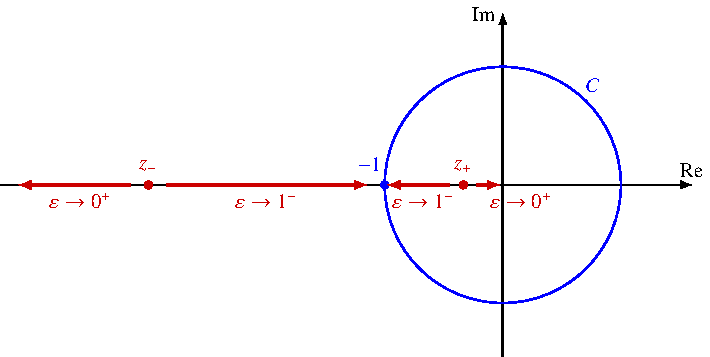
\includegraphics{papers/kepler/images/polstellen.pdf}
\caption{Lage der beiden Polstellen relativ zum Integrationsweg $C$.
Gezeichnet ist der Fall $\varepsilon=0.6$.
Beide Polstellen liegen auf der negativen reellen Achse, hier bei $z_+=-\frac13$ und $z_-=-3$.
Nur $z_+$ liegt im Inneren des Einheitskreises.
Nur dieser Pol trägt zum Wegintegral bei.
Die roten Pfeile deuten das Verhalten bei Veränderung von $\varepsilon$ an.
Für $\varepsilon\to 1^-$ streben beide Pole gegen den Punkt $-1$ auf dem Einheitskreis.
\label{kepler:figure:polstellen}}
\end{figure}


Der Wert eines Wegintegrals wird durch die Singularitäten im Inneren der Kurve bestimmt.
Wir suchen deshalb die Nullstellen des Nenners.
\index{Polstelle}%
Dazu lösen wir die quadratische Gleichung
\[
z^2+\frac{2}{\varepsilon}z+1
=
0
\qquad\Rightarrow\qquad
z_{\pm}
=
-\frac{1}{\varepsilon}\pm\!\sqrt{\frac{1}{\varepsilon^2}-1}.
\]
Wegen $0<\varepsilon<1$ ist der Radikand positiv.
Beide Nullstellen sind also reell und negativ.
Der Integrand hat in $z_+$ und $z_-$ je einen Pol zweiter Ordnung.
Auf dem Integrationsweg selbst liegen keine Pole.

Die Wurzelausdrücke sehen kompliziert aus.
Sie werden sich später aber stark vereinfachen.
Im Moment interessiert nur eine Frage: Welcher Pol liegt innerhalb von $C$?
Die Antwort auf diese Frage bekommen wir mittels Grenzwertbetrachtungen für $z_+$ und $z_-$.
Die roten Pfeile in Abbildung~\ref{kepler:figure:polstellen} zeigen, wie sich die beiden Pole dabei bewegen.

Für die Nullstelle $z_-$ gilt:
\begin{align*}
\lim_{\varepsilon \to 0^+} z_- &= \lim_{\varepsilon \to 0^+} \biggl(-\frac{1}{\varepsilon}-\!\sqrt{\frac{1}{\varepsilon^2}-1}\biggr) = -\infty, \\
\lim_{\varepsilon \to 1^-} z_- &= \lim_{\varepsilon \to 1^-} \biggl(-\frac{1}{\varepsilon}-\!\sqrt{\frac{1}{\varepsilon^2}-1}\biggr) = -1.
\end{align*}
Der Pol $z_-$ liegt also ausserhalb des Einheitskreises.

Für die Nullstelle $z_+$ verhalten sich die Grenzwerte folgendermassen:
\begin{align*}
\lim_{\varepsilon \to 0^+} z_+ &= \lim_{\varepsilon \to 0^+} \biggl(-\frac{1}{\varepsilon}+\!\sqrt{\frac{1}{\varepsilon^2}-1}\biggr) = 0, \\
\lim_{\varepsilon \to 1^-} z_+ &= \lim_{\varepsilon \to 1^-} \biggl(-\frac{1}{\varepsilon}+\!\sqrt{\frac{1}{\varepsilon^2}-1}\biggr) = -1.
\end{align*}
Wie wir sehen, liegt der Pol $z_+$ innerhalb des Einheitskreises.

Die Grenzwerte beschreiben allerdings nur die Ränder des Intervalls $0<\varepsilon<1$.
Den Nachweis für das ganze Intervall liefert der Satz von Vieta.
Nach ihm ist das Produkt der beiden Nullstellen $z_+z_-=1$.
Beide sind negativ, und wegen $z_-<z_+$ ist $|z_+|<|z_-|$.
Zusammen mit $|z_+|\,|z_-|=1$ folgt daraus $|z_+|<1<|z_-|$.
Für jede Exzentrizität $0<\varepsilon<1$ liegt also genau ein Pol im Inneren des Einheitskreises, nämlich $z_+$.

\subsection{Auswertung mit der Cauchy-Formel für Ableitungen
\label{kepler:subsection:cauchy}}

Wir wollen die Cauchy-Integralformel von
Satz~\ref{buch:integration:satz:residuensatz} anwenden, genauer ihre
Verallgemeinerung für Ableitungen.
Dazu schreiben wir den Integranden passend um.
Nur der Pol im Inneren soll noch explizit auftreten.
Mit den beiden Nullstellen $z_+$ und $z_-$ zerfällt der Nenner in die Linearfaktoren
\[
z^2+\frac{2}{\varepsilon}z+1
=
(z-z_+)(z-z_-).
\]
Damit ist
\begin{align}
\oint_C
\frac{z}{\bigl(z^2+\frac{2}{\varepsilon}z+1\bigr)^2}
\,dz
=
&
\oint_C
\frac{f(z)}{(z-z_+)^2}
\,dz
\qquad\text{mit}\qquad
f(z)
=
\frac{z}{(z-z_-)^2}.
\notag
\intertext{Die Funktion $f$ ist auf dem Einheitskreis und in seinem Inneren holomorph.
Ihre einzige Singularität $z_-$ liegt nämlich ausserhalb.
Der Pol in $z_+$ ist von zweiter Ordnung.
Wir brauchen deshalb die Cauchy-Formel für Ableitungen aus Satz~\ref{buch:integration:satz:ableitungn}.
\index{Cauchy-Integralformel}%
Für $n=1$ liefert sie}
&
\oint_C
\frac{f(z)}{(z-z_+)^2}
\,dz
=
2\pi i\,f'(z_+).
\label{kepler:eqn:ableitungsformel}
\end{align}
Das Wegintegral ist damit auf eine einzige Ableitung zurückgeführt.
\index{Wegintegral}%
Mit der Quotientenregel finden wir
\begin{align*}
f'(z)
&=
\frac{(z-z_-)^2-2z(z-z_-)}{(z-z_-)^4}
=
\frac{(z-z_-)-2z}{(z-z_-)^3}
=
-\frac{z+z_-}{(z-z_-)^3}.
\intertext{Jetzt setzen wir die Stelle $z_+$ ein.
Zähler und Nenner lassen sich direkt durch die Vieta-Beziehungen der quadratischen Gleichung $z^2+\smash{\frac{2}{\varepsilon}}z+1=0$ ausdrücken.
\index{Vieta-Beziehungen}%
Im Zähler steht die Summe $z_++z_-=-2/\varepsilon$.
Im Nenner steht die Differenz $z_+-z_-=2\smash{\sqrt{1/\varepsilon^2-1}}$.
Die unhandlichen Wurzelterme kombinieren sich dadurch zu}
f'(z_+)
&=
-\frac{z_++z_-}{(z_+-z_-)^3}
=
\frac{2/\varepsilon}{8\bigl(\frac{1}{\varepsilon^2}-1\bigr)^{\frac{3}{2}}}
=
\frac{1}{4\varepsilon}
\cdot
\biggl(\frac{\varepsilon^2}{1-\varepsilon^2}\biggr)^{\frac{3}{2}}
=
\frac{\varepsilon^2}{4\,(1-\varepsilon^2)^{\frac{3}{2}}}.
\end{align*}
Dieses Resultat setzen wir über \eqref{kepler:eqn:ableitungsformel}
in \eqref{kepler:eqn:wegintegral} ein.
Der Faktor $\varepsilon^2$ und die imaginäre Einheit heben sich weg.
Es bleibt der reelle Wert
\begin{equation}
\int_0^{2\pi}
\frac{1}{(1+\varepsilon\cos(\vartheta))^2}
\,d\vartheta
=
\frac{4}{i\varepsilon^2}
\cdot
2\pi i
\cdot
\frac{\varepsilon^2}{4\,(1-\varepsilon^2)^{\frac{3}{2}}}
=
\frac{2\pi}{(1-\varepsilon^2)^{\frac{3}{2}}}.
\label{kepler:eqn:integralwert}
\end{equation}
Am Ende kommt also eine reelle Zahl heraus.
Das ist eine willkommene Kontrolle, denn das Ausgangsintegral war reell.
Auch der Grenzfall stimmt.
Für $\varepsilon\to 0$ liefert \eqref{kepler:eqn:integralwert} den Wert $2\pi$.
Denselben Wert haben wir in
Abschnitt~\ref{kepler:subsection:integralspezialfall} für die
Kreisbahn direkt berechnet.

\subsection{Das dritte keplersche Gesetz
\label{kepler:subsection:resultat}}

Jetzt setzen wir alles zusammen.
Mit dem Integralwert \eqref{kepler:eqn:integralwert} wird aus der
Umlaufzeit \eqref{kepler:eqn:tintegral}
\begin{align}
T
&=
\frac{m\,p^2}{L}
\cdot
\frac{2\pi}{(1-\varepsilon^2)^{\frac{3}{2}}}.
\notag
\intertext{Den Drehimpuls ersetzen wir mit
\eqref{kepler:eqn:drehimpulsgeometrie} durch $L=m\sqrt{GMp\mathstrut}$.
Die Planetenmasse $m$ kürzt sich dabei wie schon im Kreisfall heraus:}
T
&=
\frac{p^2}{\!\sqrt{GMp\mathstrut}}
\cdot
\frac{2\pi}{(1-\varepsilon^2)^{\frac{3}{2}}}
=
\frac{2\pi}{\!\sqrt{GM\mathstrut\rlap{$\phantom{p}$}}}
\cdot
\frac{p^{\frac{3}{2}}}{(1-\varepsilon^2)^{\frac{3}{2}}}.
\notag
\intertext{Nach \eqref{kepler:eqn:ellipse} ist $p=a(1-\varepsilon^2)$.
Der Faktor $(1-\varepsilon^2)$ fällt damit vollständig aus der Formel heraus:}
T
&=
\frac{2\pi}{\!\sqrt{GM\mathstrut\rlap{$\phantom{p}$}}}
\cdot
\frac{a^{\frac{3}{2}}(1-\varepsilon^2)^{\frac{3}{2}}}{(1-\varepsilon^2)^{\frac{3}{2}}}
=
\frac{2\pi\,a^{\frac{3}{2}}}{\!\sqrt{GM\mathstrut\rlap{$\phantom{p}$}}}.
\notag
\intertext{Die Umlaufzeit hängt also weder von der Masse des Planeten noch von der Exzentrizität seiner Bahn ab.
Sie hängt nur von der grossen Halbachse und der Masse des Zentralgestirns ab.
Quadrieren liefert das dritte keplersche Gesetz in seiner üblichen Form
\index{keplersches Gesetz!drittes}}
\frac{T^2}{a^3}
&=
\frac{4\pi^2}{GM}
=
\text{konstant}.
\label{kepler:eqn:keplerdrei}
\end{align}
Für $\varepsilon=0$ und $a=r$ enthält es das Resultat
\eqref{kepler:eqn:kreisbahn} für Kreisbahnen als Spezialfall.

\subsection{Plausibilisierung anhand realer Bahndaten
\label{kepler:subsection:plausibilisierung}}

\begin{table}
\centering
\begin{tabular}{lrrrr}
Körper & $\varepsilon$ & $a$ in $\text{m}$ & $T$ in $\text{s}$
& $T^2/a^3$ in $\text{s}^2\text{m}^{-3}$
\\
\hline
Erde   & $0.017$ & $1.496\cdot 10^{11}$ & $3.156\cdot 10^{7}$
& $2.975\cdot 10^{-19}$
\\
Mars   & $0.094$ & $2.279\cdot 10^{11}$ & $5.935\cdot 10^{7}$
& $2.976\cdot 10^{-19}$
\\
67P    & $0.641$ & $5.180\cdot 10^{11}$ & $2.033\cdot 10^{8}$
& $2.974\cdot 10^{-19}$
\end{tabular}
\caption{Bahndaten der Erde, des Mars und des Kometen
67P/Tschurjumow-Gerassimenko nach \cite{kepler:nasafactsheet} und
\index{Erde}%
\index{Mars}%
\index{67P/Tschurjumow-Gerassimenko}%
\index{Tschurjumow-Gerassimenko}%
\cite{kepler:jplsbdb}.
Die Exzentrizitäten $\varepsilon$ der drei Körper sind sehr unterschiedlich.
Trotzdem stimmt der Quotient $T^2/a^3$ überall auf drei Stellen mit
dem theoretischen Wert
$4\pi^2/GM_{\odot}=2.975\cdot 10^{-19}\,\text{s}^2\text{m}^{-3}$
überein.
\label{kepler:table:plausibilisierung}}
\end{table}

Zum Schluss prüfen wir das Resultat \eqref{kepler:eqn:keplerdrei} an realen Daten.
Tabelle~\ref{kepler:table:plausibilisierung} vergleicht die Erde, den Mars und den Kometen 67P/Tschurjumow-Gerassimenko.
Der Komet ist durch die Rosetta-Mission bekannt geworden.
Als Testfall ist er besonders interessant.
Seine Bahn hat die Exzentrizität $\varepsilon\approx 0.641$.
Sie ist damit weit von einer Kreisbahn entfernt.
Die Kreisbahn-Herleitung aus Abschnitt~\ref{kepler:subsection:kraeftegleichgewicht} macht über ihn deshalb keine Aussage.
Die Bahndaten stammen aus \cite{kepler:nasafactsheet} und \cite{kepler:jplsbdb}.
Für die Sonne gilt $GM_{\odot}=1.327\cdot 10^{20}\,\text{m}^3\text{s}^{-2}$.
Damit ergibt sich für alle drei Körper derselbe Quotient $T^2/a^3$.
Er stimmt mit dem theoretischen Wert $4\pi^2/GM_{\odot}$ überein.

Das dritte keplersche Gesetz ist damit für beliebige elliptische Bahnen bewiesen und numerisch bestätigt.
Die Unabhängigkeit von der Planetenmasse macht es zu einem praktischen Werkzeug.
Man misst die Umlaufzeit und die Halbachse eines einzigen Begleiters.
Daraus liefert \eqref{kepler:eqn:keplerdrei} die Masse des Zentralkörpers.
So bestimmt man die Masse der Sonne, eines Planeten mit Monden oder eines fernen Sterns mit Exoplaneten.
Aus Sicht dieses Seminars ist vor allem der Weg bemerkenswert.
Am Anfang stand ein reelles Integral, an dem sich die Schulanalysis die Zähne ausbeisst.
In der komplexen Ebene zerfiel es in drei einfache Schritte: eine Substitution, eine quadratische Gleichung und eine einzige Ableitung.


\printbibliography[heading=subbibliography]
\end{refsection}
